\begin{frame}
    \frametitle{Nash Equilibrium}
    \centering

    \scriptsize
    \begin{equation*}
        R =  
        \begin{pmatrix}
            0.5 & 0.1 & 0 & 0 \\
            0.9 & 0.5 & 0.2 & 0 \\
            1 & 0.8 & 0.5 & 0.3 \\
            1 & 1 & 0.7 & 0.5
        \end{pmatrix}
    \end{equation*}
    \begin{equation*}
        A = 
        \begin{pmatrix}
            0.99998394 & 0.99998394 & 0.99998394 & 0.99998394 \\
            0.99998955 & 0.99998848 & 0.99998649 & 0.9999845 \\
            0.99999952 & 0.9999987  & 0.99999596 & 0.99999199 \\
            0.99994372 & 0.99995113 & 0.99998603 & 0.99999911
        \end{pmatrix}
    \end{equation*}
    \begin{equation*}
        B = 
        \begin{pmatrix}
            0.99998394 & 0.99998955 & 0.99999952 & 0.99994372 \\
            0.99998394 & 0.99998848 & 0.9999987  & 0.99995113 \\
            0.99998394 & 0.99998649 & 0.99999596 & 0.99998603 \\
            0.99998394 & 0.9999845  & 0.99999199 & 0.99999911 \\
        \end{pmatrix}
    \end{equation*}

    \begin{equation*}
        \textbf{Nash Equilibria: } 
        \begin{array}{cc}
            \underline{\quad A \quad} & \underline{\quad B \quad} \\
            % (0, 0, 1, 0) & (0, 0, 1, 0) \\ 
            % (0, 0, 0, 1) & (0, 0, 0, 1) \\ 
            (0, 0, 0.4, 0.6) & (0, 0, 0.4, 0.6) 
        \end{array}
    \end{equation*}
\end{frame}


\begin{frame}
    \frametitle{Asymmetric Replicator Dynamics}
    \centering

    \[
        \frac{dx}{dt}_i = x_i((f_x)_i - \phi_x), \quad \text{ for all }i
    \]
    \[
        \frac{dy}{dt}_i = y_i((f_y)_i - \phi_y), \quad \text{ for all }i
    \]
    
\end{frame}


\begin{frame}
    \frametitle{Inefficiency measure}

    \begin{equation*}
        PoA = \frac{\max_{s \in E} Cost(s)}{\min_{s \in S} Cost(S)}
    \end{equation*}
    \pause
    \footnotesize
    \vspace{1cm}
    \begin{equation*}
        PoA_A(s_r) = \frac{Cost(s_r)}{\min_{s \in S} Cost(S)}, \hspace{1cm} 
        PoA_B(s_c) = \frac{Cost(s_c)}{\min_{s \in S} Cost(S)}
    \end{equation*}
\end{frame}


\begin{frame}
    \frametitle{Learning algorithms - Asymmetric replicator dynamics}

    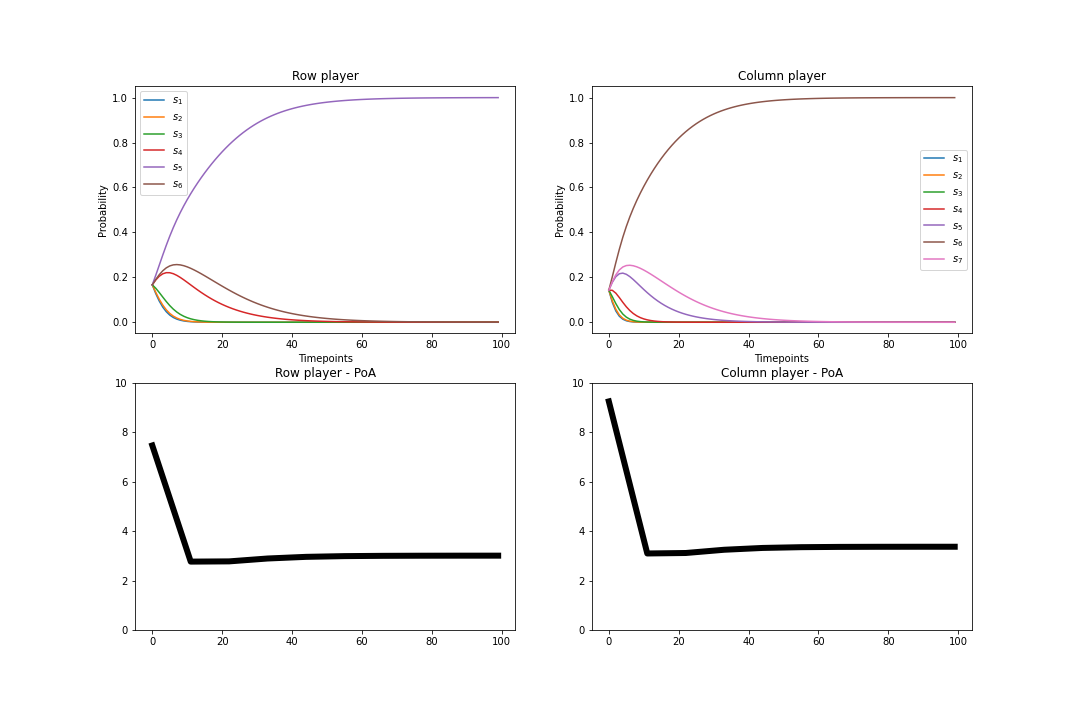
\includegraphics[scale=0.28]{Bin/ARD_game.png}
\end{frame}

\begin{frame}
    \centering
    \Huge{
    Inefficiencies can be learned and emerge naturally
    }
\end{frame}


\begin{frame}
    \frametitle{Learning algorithms - Asymmetric replicator dynamics}

    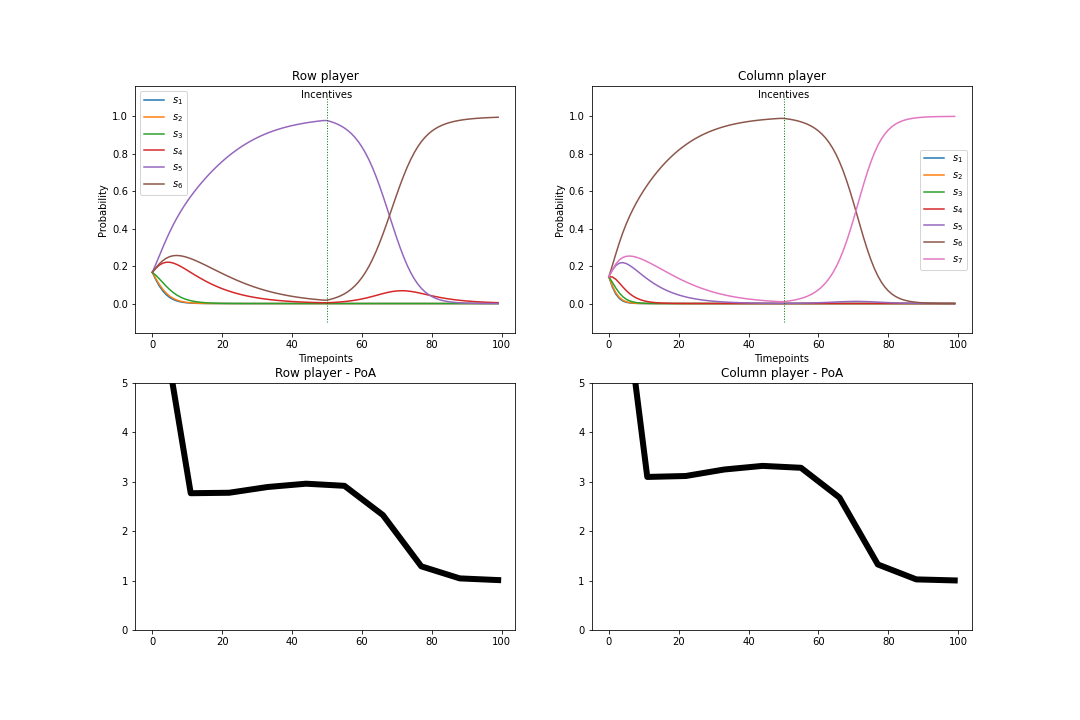
\includegraphics[scale=0.28]{Bin/ARD_penalty_game.png}
    
\end{frame}


\begin{frame}
    \centering
    \Huge{
    Targeted incentivisation of behaviours can help escape learned inefficiencies
    }
\end{frame}
